\documentclass[submission]{eptcs}
\providecommand{\event}{TTC 2014}

\usepackage[T1]{fontenc}
\usepackage{url}
\usepackage{hyperref}
\usepackage[cache]{minted}
\newminted{clojure}{fontsize=\fontsize{8}{8},linenos,numbersep=3pt}
\newminted{java}{fontsize=\fontsize{8}{8},linenos,numbersep=3pt}
\newmintinline{clojure}{fontsize=\footnotesize}
\newmintinline{java}{fontsize=\fontsize{8}{8}}
\newmintinline{xml}{fontsize=\fontsize{8}{8}}
\newmintinline{c}{fontsize=\fontsize{8}{8}}
\newminted{csharp}{frame=lines,fontsize=\fontsize{8}{8},linenos,numbersep=3pt}
\newminted{cpp}{frame=lines,fontsize=\fontsize{8}{8},linenos,numbersep=3pt}
\newminted{c}{frame=lines,fontsize=\fontsize{8}{8},linenos,numbersep=3pt}
\newmintedfile{xml}{frame=lines,fontsize=\fontsize{8}{8},linenos,numbersep=3pt}
\newcommand{\code}{\clojureinline}
\usepackage{paralist}
\usepackage{graphicx}

\usepackage[skip=0pt]{caption}

\setlength{\abovecaptionskip}{0ex}
\setlength{\belowcaptionskip}{-10pt}

\title{Solving the TTC FIXML Case with FunnyQT}
\author{Tassilo Horn
  \institute{Institute for Software Technology, University Koblenz-Landau, Germany}
  \email{horn@uni-koblenz.de}}

\def\titlerunning{Solving the TTC FIXML Case with FunnyQT}
\def\authorrunning{T. Horn}

\begin{document}
\maketitle

\begin{abstract}
  FunnyQT is a model querying and model transformation library for the
  functional Lisp-dialect Clojure providing a rich and efficient querying and
  transformation API.  This paper describes the FunnyQT solution to the TTC
  2014 FIXML transformation case.  It solves the core task of generating Java,
  C\#, C++, and C code for a given FIXML message.  It also solves the extension
  tasks of determining reasonable types for the fields of classes.
\end{abstract}


\section{Introduction}
\label{sec:introduction}

This paper describes the FunnyQT solution of the TTC 2014 FIXML
Case~\cite{fixml-case-desc} which solves the core task of generating Java, C\#,
and C++ code for a given FIXML messages.  It also solves the extension task of
heuristically determining appropriate types for the fields of the generated
classes and the extension task to generate non-object-oriented C code.  The
solution also sports several features that were not requested.  For example, if
an XML element has multiple children with the same tag, then the corresponding
class or struct will have a field being an array of the type corresponding to
the tag instead of multiple numbered fields.  For C++ and C, proper
destructors/recursive freeing functions are generated, and the classes/structs
are declared in a header and defined in a separate implementation file.  For
all languages, proper import/include/using-statements are generated, and the
code compiles without warnings using the standard compilers for the respective
language (GCC, Mono, Java).

The solution allows to create a data model given a single FIXML message as
requested by the case description, but it can also be \emph{run on arbitrary
  many FIXML messages at once}.  The idea is that with a reasonable large
number of sample messages, the transformation is able to produce a more
accurate data model.  By having more samples, optional attributes and child
elements are more likely to be identified.  Similarly, child elements which
usually occur only once but may in fact occur multiple times are more likely to
be identified.  And finally, the heuristical detection of an appropriate field
type benefits from more sample data, too.

Section~\ref{sec:posrpt} in the appendix on page~\pageref{sec:posrpt} shows the
code which was generated for the FIXML position report message
\texttt{test2.xml}.

FunnyQT~\cite{Horn2013MQWFQ} is a model querying and transformation library for
the functional Lisp dialect Clojure.  Queries and transformations are plain
Clojure programs using the features provided by the FunnyQT API.  This API is
structured into several task-specific sub-APIs/namespaces, e.g., there is a
namespace containing constructs for writing polymorphic functions dispatching
on metamodel type, a namespace containing constructs for model-to-model
transformations, etc.

The solution project is available on
Github\footnote{\url{https://github.com/tsdh/ttc14-fixml}}, and it is set up
for easy reproduction on
SHARE\footnote{\url{http://is.ieis.tue.nl/staff/pvgorp/share/?page=ConfigureNewSession&vdi=Ubuntu12LTS_TTC14_64bit_FunnyQT4.vdi}}.

\section{Solution Description}
\label{sec:solution-description}

In this section, the transformation specification for all three main tasks is
going to be explained.

\subsection{Task 1: XML to Model}
\label{sec:xml2model}

Since handling XML files is a common task, FunnyQT already ships with a
namespace \emph{funnyqt.xmltg} which contains a transformation function
\code|xml2xml-graph| from XML files to a DOM-like model conforming to a
detailed XML metamodel which also supports XML namespaces.  This function uses
Java's \emph{Stream API for XML} (\emph{StAX}) under the hoods, so XML files
that aren't well-formed lead to parsing errors.


\subsection{Task 2: XML Model to OO Model}
\label{sec:xml-to-oo}

Core task~2 deals with transforming the XML models into models conforming to a
metamodel suited for object-oriented languages.  The metamodel used by the
FunnyQT solution is shown in Figure~\ref{fig:oo-mm}.

\begin{figure}[h!t]
  \centering
  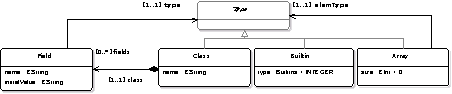
\includegraphics[width=\textwidth]{../postproc/oo-mm}
  \caption{The OO metamodel}
  \label{fig:oo-mm}
\end{figure}

FunnyQT contains a feature for generating metamodel-specific APIs which is used
here.  The generated XML and OO APIs are referred to by the namespace aliases
\code|xml| and \code|oo| in the listings below.  They contain getter and setter
functions for attributes (e.g., \code|(xml/set-name! el val)|), role name
accessor functions (e.g., \code|(oo/->fields cls)|), and several more.

In FunnyQT, a model-to-model transformation is specified using the
\code|deftransformation| macro.  It receives the name of the transformation,
and a vector defining input and output models plus additional parameters.  In
this case, there is only one single input model \code|xml|, one single output
model \code|oo|.

\begin{clojurecode*}{numbers=none}
(deftransformation xml-graph2oo-model [[xml] [oo]]
  ...)
\end{clojurecode*}

Inside such a transformation definition, arbitrary many rule and helper
function definitions may occur.  The first rule of the transformation is
\code|element2class| shown in the next listing.

\begin{clojurecode*}{numbers=none}
  (^:top element2class
   :from [e '[:and Element !RootElement]]
   :to   [c (element-name2class (xml/name e))])
\end{clojurecode*}

The \code|^:top| annotation defines this rule as a top-level rule being applied
automatically.  The \code|:from| clause restricts the elements \code|e| this
rule is applicable for to those of metamodel type \code|Element| but not of
type \code|RootElement|.  The reason is that we don't want to create a class
for the \texttt{FIXML} element which is the root element of any FIXML message.

The \code|:to| clause defines which elements should be created for matching
elements.  Usually, it would be specified as \code|:to [x 'SomeClass]| in which
case \code|x| would be a new element of type \code|SomeClass|.  However, in the
current case, there is no one-to-one mapping between XML elements and OO
classes, because the XML model may contain multiple elements with the same tag
name, and there should be exactly one OO class per unique tag name.  Therefore,
the \code|:to| clause delegates the creation of class \code|c| to another rule
\code|element-name2class| providing \code|e|'s tag name as argument.

When a rule is applied to an input element for which its \code|:from| clause
matches, target elements are created according to its \code|:to| cause.  The
mapping from input to output elements is saved.  When a rule gets applied to an
element it has already been applied to, the elements that have been created by
the first call are returned instead of creating new elements.

The \code|element-name2class| rule shown below receives as input a plain
string, the \code|tag-name| of an element, and it creates a \code|Class c| in
the target model.  The name of the class corresponds to the \code|tag-name|.
According to the rule semantics sketched above and the fact that this rule gets
called with the tag name of any element by \code|element2class|, there will be
one target class for every unique tag name.

\begin{clojurecode*}{numbers=none}
  (element-name2class
   :from [tag-name]
   :to   [c 'Class {:name tag-name}]
   (doseq [[an at av] (all-attributes tag-name)]
     (attribute2field an at av c))
   (doseq [[tag max-child-no] (all-children tag-name)]
     (children-of-same-tag2field tag max-child-no c))
   (when-let [char-conts (seq (all-character-contents tag-name))]
     (character-contents2field char-conts c)))
\end{clojurecode*}

Following the \code|:from| and \code|:to| clauses comes the rule's body where
arbitrary code may be written.  Here, three other rules \code|attribute2field|,
\code|children-of-same-tag2field|, and \code|character-contents2field| are
called for all XML attributes, child elements, and character
contents\footnote{The case description doesn't demand that XML character
  content should be handled.  However, without handling them transforming
  \texttt{test3.xml} and \texttt{test4.xml} would lead to several classes
  without any fields.}  of element \code|e|.  These rules and the helpers
\code|all-attributes|, \code|all-children|, and \code|all-character-contents|
are skipped for brevity but they follow the same style and mechanics.

The next listing shows the helper implementing the extension task of
heuristically determining an appropriate field type from XML attribute values.

\begin{clojurecode*}{numbers=none}
  (guess-type [vals]
   (let [ts (set (map #(condp re-matches %
                         #"\d\d\d\d-\d\d-\d\d.*" DATE
                         #"[+-]?\d+\.\d+"        DOUBLE
                         #"[+-]?\d+"             (int-type %)
                         STRING) vals))]
     (get-or-create-builtin-type
      (cond (= (count ts) 1)              (first ts)
            (= ts #{DOUBLE INTEGER})      DOUBLE
            (= ts #{DOUBLE LONG})         DOUBLE
            (= ts #{DOUBLE LONG INTEGER}) DOUBLE
            (= ts #{INTEGER LONG})        LONG
            :else                         STRING))))
\end{clojurecode*}

The \code|guess-type| function receives a collection \code|vals|.  \code|vals|
could either be all character contents of an XML element, or all attribute
values of an attribute that occurs in many XML elements of the same tag.  Every
given value is checked against a regular expression that determines its type
being either a timestamp in ISO 8601 notation, a double value, or an integer
value.  If none match, then \code|STRING| is used as its type.  In case of an
integer value, the function \code|int-type| further determines if the value can
be represented as a 32 bit integer, or if a 64 bit long is needed.

The \code|cond| expression picks the type that can be used to represent all
values.  If all values are guessed to be of the very same type, then this type
is chosen.  For multiple numeric types, the respective ``largest'' type is
chosen where \code|INTEGER| < \code|LONG| < \code|DOUBLE|.  Else, we fall back
to \code|STRING|.  The picked type is then passed to the rule
\code|get-or-create-builtin-type| which creates a \code|Builtin| whose
\code|type| attribute is set to the type determined by the \code|cond|
expression.

The complete \code|xml-graph2oo-model| transformation consists of 6 rules and 7
helpers amounting to 70 LOC.  The result is an OO model whose field elements
already have the heuristically guessed types, and where multiple-occuring XML
child elements of the same type where compressed to array fields.


\subsection{Task 3: OO Model to Code}
\label{sec:oo-model-to-code}

The last step of the overall transformation is to generate code in different
programming languages from the OO model created in the previous step.  In
addition to the core task languages, the FunnyQT solution also generates C code
as an extension.

One crucial benefit of FunnyQT being a Clojure library is that we can simply
use arbitrary other Clojure and Java libraries for our needs.  So for this
task, we use the excellent
\emph{Stencil}\footnote{\url{https://github.com/davidsantiago/stencil}}
library.  Stencil is a Clojure templating library implementing the popular,
lightweight \emph{Mustache}
specification\footnote{\url{http://mustache.github.io/}}.  The idea of Mustache
is that one defines a template file containing placeholders which can be
rendered to a concrete file by providing a map where the keys are the
placeholder names and the values are the text that should be substituted.
There are also placeholders for collections in which case the corresponding
value of the map has to be a collection of maps.  We'll discuss the solution
using the template for Java.

\begin{javacode*}{numbers=none}
package {{{pkg-name}}};
{{#imports}}import {{{imported-class}}};{{/imports}}
class {{{class-name}}} {
    {{#fields}}
    private {{{field-type}}} {{{field-name}}};
    {{/fields}}
    public {{{class-name}}}() {
        {{#fields}}
        this.{{{field-name}}} = {{{field-value-exp}}};
        {{/fields}}
    } /* parametrized constructor, getters, and setters elided... */ }

\end{javacode*}

So a map to feed to the Stencil templating engine needs to provide the keys
\code|:pkg-name|, \code|:imports|, \code|:class-name|, etc.  The values for the
\code|:imports| and \code|:fields| keys need to be collections of maps
representing one import or field each, e.g., a field is represented as a map
with keys \code|:field-type|, \code|:field-name|, and
\code|:field-value-expression|.

The templates for the other languages use the same keys (although there are
some keys in the C and C++ templates that are only needed by them), so the
essential job of the code generation task is to derive such a map for every
class in our OO model that can then be passed to Stencil's rendering function.

This is done using a FunnyQT polymorphic function \code|to-mustache| whose
definition is given below.

\begin{clojurecode}
(declare-polyfn to-mustache [el lang pkg])
(defpolyfn to-mustache oo.Class [cls lang pkg]
  {:pkg-name pkg
   :imports (get-imports cls lang)
   :class-name (oo/name cls)
   :fields (mark-first-field (map #(to-mustache % lang pkg) (oo/->fields cls)))})
(defpolyfn to-mustache oo.Field [f lang pkg]
  {:field-type (field-type (oo/->type f) lang)
   :field-name (oo/name f)
   :field-value-exp (field-value-exp f lang)
   :plain-field-type (let [t (oo/->type f)]
                       (type-case t
                         'Array (oo/name (oo/->elemType t))
                         'Class (oo/name t)
                         nil))})
\end{clojurecode}

A polymorphic function in FunnyQT is a function that dispatches between several
implementations based on the metamodel type of its first argument.  They can be
seen as a kind of object-oriented method attached to metamodel classes.  Line 1
declares the polymorphic function \code|to-mustache| and defines that it gets
three parameters: an OO model element \code|el|, the target language
\code|lang|, and the package/namespace name \code|pkg| in which the
class/struct should be generated.  Lines 2 to 6 then define an implementation
for elements of the metamodel class \code|Class|, and lines 7-18 define an
implementation for elements of metamodel class \code|Field|.  Both
implementations call several helper functions that query the OO model to
compute the relevant values for the map's keys which are skipped for brevity
here.


\section{Evaluation and Conclusion}
\label{sec:evaluation}

The \emph{complexity} should be measured as the sum of number of operator
occurrences and feature and entity type name references.  The FunnyQT solution
contains about 300 expressions, 24 metamodel type references, and 18 property
references resulting in a complexity of 342.  So it is quite complex but it
does much more than what was required.  A solution soving only the required
tasks would have the same amount of metamodel type and property references but
would be approximately one third shorter.

\emph{Accuracy} should measure the degree of syntactical correctness of the
generated code and the degree of how well it matches the source FIXML messages.
The FunnyQT solution has a very high accuracy.  The code is correct and
compiles without warnings.  It also matches the source FIXML messages well.
The creation of one array field for multiple XML children with the same tag is
better than creating several separate fields.  Guessing appropriate types for
the fields instead of always using string improves the usefulness of the
generated code.  Also, that the transformation can be run on an arbitrarily
large sample of FIXML messages in one go improves the accuracy even more.

The overall \emph{development time} of the solution can be estimated with about
8 person-hours for the core task and 4 more hours to generalize and extend it
to the final version.

Since FunnyQT's generic \code|xml2xml-graph| transformation uses Java's StAX
API internally, the \emph{fault tolerance} is high.  Documents which are not
well-formed lead to parsing errors.

The \emph{execution time} is good.  For all provided test models, the complete
transformation including parsing XML, transforming the XML model to an OO model
followed by generating code in all four languages took at most 700 milliseconds
on SHARE.  Running the transformation on all provided and five additional FIXML
messages at once took about 1.5 seconds.

The \emph{modularity} of the \code|xml-graph2oo-model| is
\(Mod = 1 - \frac{d}{r} = 1 - \frac{5}{6} = 0.1\overline{6}\)
where \(r\)
is the number of rules and \(d\)
is the number of dependencies between them.  The code generation is implemented
with 10 functions that call each other.  Since some functions are recursive and
called from different places 12 call dependencies can be counted.  Thus, the
modularity is \(Mod = 1 - \frac{12}{10} = -0.2\).


With respect to \emph{abstraction level}, the \code|xml-graph2oo-model|
transformation is quite low-level. The code generation is split into
declarative templates, and functions that derive a map of template placeholder
keywords to the values that have to be filled in for each class.  Those
functions are all pure functional.  Thus, the abstraction level of the FunnyQT
solution is about medium.


\bibliographystyle{alpha}
\bibliography{ttc-fixml}

\newpage
\appendix

\section{Transformation of a Position Report Message}
\label{sec:posrpt}

In this section, the stepwise outcomes of transforming a position report
message (\texttt{test2.xml}) are illustrated.

The FIXML document itself is printed in Section~\ref{sec:posrpt:xml}.

Section~\ref{sec:posrpt:xml-graph} shows its representation as an FunnyQT XML
model.  This part of the overall transformation has been discussed in
Section~\ref{sec:xml2model}.

Section~\ref{sec:posrpt:oo} shows the OO model conforming to the metamodel
shown in Figure~\ref{fig:oo-mm} which is generated by the
\code|xml-graph2oo-model| transformation discussed in
Section~\ref{sec:xml-to-oo}.

Finally, the sections \ref{sec:posrpt:java}, \ref{sec:posrpt:csharp},
\ref{sec:posrpt:cpp}, and \ref{sec:posrpt:c} show the source code files for the
\code|PosRpt| class and the \code|Util| class which contains helpers for the
data model classes.  For Java and C\#, there is only one source code file for
the \code|PosRpt| class whereas for C++ and C, the class/struct is declared in
a header file and its definition is held in a separate implementation file.  It
should be noted that all source code files are printed here exactly as produced
by the transformation.  No additional formatting has been done, and they all
compile without warnings using standard compilers for the languages, i.e.,
\code|javac| from the OpenJDK project\footnote{\url{http://openjdk.java.net/}}
for Java, \code|mcs| from the Mono
project\footnote{\url{http://www.mono-project.com}} for C\#, and
\code|g++|/\code|gcc| from the GNU Compiler
Collection\footnote{\url{http://gcc.gnu.org/}} for C++ and C.  However, the C++
code uses extended initializer lists which are new in the C++11 standard, so a
\code|-std=c++0x| (or \code|-std=c++11|) has to be added to the \code|g++| call
in order not to get warnings.


\subsection{The Position Report as XML document}
\label{sec:posrpt:xml}

\xmlfile{../messages/test2.xml}

\newpage
\subsection{The Position Report as XML Graph}
\label{sec:posrpt:xml-graph}
\begin{center}
  
\includegraphics[angle=90,height=.95\textheight]{xml-test2}
\end{center}

\newpage
\subsection{The Position Report as OO Model}
\label{sec:posrpt:oo}
\begin{center}
  
\includegraphics[angle=90,height=.95\textheight]{oo-test2}
\end{center}

\newpage
\subsection{The Position Report as Java Class}
\label{sec:posrpt:java}

\paragraph{PosRpt.java}
\begin{javacode}
package test2;

import java.util.Date;

class PosRpt {
    private int ReqTyp;
    private String Ccy;
    private int Rslt;
    private int AcctTyp;
    private int SetPxTyp;
    private double PriSetPx;
    private int RptID;
    private double SetPx;
    private Date BizDt;
    private int Acct;
    private Amt Amt_obj;
    private Instrmt Instrmt_obj;
    private Qty[] Qty_objs;
    private Pty[] Pty_objs;
    private Hdr Hdr_obj;

    public PosRpt() {
        this.ReqTyp = 0;
        this.Ccy = "USD";
        this.Rslt = 0;
        this.AcctTyp = 1;
        this.SetPxTyp = 1;
        this.PriSetPx = 0.00;
        this.RptID = 541386431;
        this.SetPx = 0.00;
        this.BizDt = Util.parseDate("2003-09-10T00:00:00");
        this.Acct = 1;
        this.Amt_obj = new Amt();
        this.Instrmt_obj = new Instrmt();
        this.Qty_objs = new Qty[] {new Qty(), new Qty(), new Qty()};
        this.Pty_objs = new Pty[] {new Pty(), new Pty(), new Pty()};
        this.Hdr_obj = new Hdr();
    }

    public PosRpt(int ReqTyp, String Ccy, int Rslt, int AcctTyp, int SetPxTyp, double PriSetPx, int RptID,
                  double SetPx, Date BizDt, int Acct, Amt Amt_obj, Instrmt Instrmt_obj, Qty[] Qty_objs,
                  Pty[] Pty_objs, Hdr Hdr_obj) {
        this.ReqTyp = ReqTyp;
        this.Ccy = Ccy;
        this.Rslt = Rslt;
        this.AcctTyp = AcctTyp;
        this.SetPxTyp = SetPxTyp;
        this.PriSetPx = PriSetPx;
        this.RptID = RptID;
        this.SetPx = SetPx;
        this.BizDt = BizDt;
        this.Acct = Acct;
        this.Amt_obj = Amt_obj;
        this.Instrmt_obj = Instrmt_obj;
        this.Qty_objs = Qty_objs;
        this.Pty_objs = Pty_objs;
        this.Hdr_obj = Hdr_obj;
    }

    public int getReqTyp() {
        return ReqTyp;
    }

    public void setReqTyp(int ReqTyp) {
        this.ReqTyp = ReqTyp;
    }

    // Other getters/setters elided...
}
\end{javacode}

\paragraph{Util.java}

\begin{javacode}
package test2;

import java.text.SimpleDateFormat;
import java.text.ParseException;
import java.util.Date;

class Util {
    private static final SimpleDateFormat dateFormat
        = new SimpleDateFormat("yyyy-MM-dd'T'HH:mm:ssXXX");

    public static Date parseDate(String date) {
        try {
            return dateFormat.parse(date);
        } catch (ParseException e) {
            throw new RuntimeException(e);
        }
    }
}
\end{javacode}


\subsection{The Position Report as C\# Class}
\label{sec:posrpt:csharp}

\paragraph{PosRpt.cs}

\begin{csharpcode}
using System;

namespace test2{
  class PosRpt {
    public int _ReqTyp { get; set; }
    public string _Ccy { get; set; }
    public int _Rslt { get; set; }
    public int _AcctTyp { get; set; }
    public int _SetPxTyp { get; set; }
    public double _PriSetPx { get; set; }
    public int _RptID { get; set; }
    public double _SetPx { get; set; }
    public DateTime _BizDt { get; set; }
    public int _Acct { get; set; }
    public Amt _Amt_obj { get; set; }
    public Instrmt _Instrmt_obj { get; set; }
    public Qty[] _Qty_objs { get; set; }
    public Pty[] _Pty_objs { get; set; }
    public Hdr _Hdr_obj { get; set; }

    public PosRpt() {
      this._ReqTyp = 0;
      this._Ccy = "USD";
      this._Rslt = 0;
      this._AcctTyp = 1;
      this._SetPxTyp = 1;
      this._PriSetPx = 0.00;
      this._RptID = 541386431;
      this._SetPx = 0.00;
      this._BizDt = Util.parseDate("2003-09-10T00:00:00");
      this._Acct = 1;
      this._Amt_obj = new Amt();
      this._Instrmt_obj = new Instrmt();
      this._Qty_objs = new Qty[] {new Qty(), new Qty(), new Qty()};
      this._Pty_objs = new Pty[] {new Pty(), new Pty(), new Pty()};
      this._Hdr_obj = new Hdr();
    }

    public PosRpt(int ReqTyp, string Ccy, int Rslt, int AcctTyp, int SetPxTyp, double PriSetPx, int RptID,
                  double SetPx, DateTime BizDt, int Acct, Amt Amt_obj, Instrmt Instrmt_obj, Qty[] Qty_objs,
                  Pty[] Pty_objs, Hdr Hdr_obj) {
      this._ReqTyp = ReqTyp;
      this._Ccy = Ccy;
      this._Rslt = Rslt;
      this._AcctTyp = AcctTyp;
      this._SetPxTyp = SetPxTyp;
      this._PriSetPx = PriSetPx;
      this._RptID = RptID;
      this._SetPx = SetPx;
      this._BizDt = BizDt;
      this._Acct = Acct;
      this._Amt_obj = Amt_obj;
      this._Instrmt_obj = Instrmt_obj;
      this._Qty_objs = Qty_objs;
      this._Pty_objs = Pty_objs;
      this._Hdr_obj = Hdr_obj;
    }
  }
}
\end{csharpcode}

\paragraph{Util.cs}

\begin{csharpcode}
using System;
using System.Globalization;

namespace test2 {
  class Util {
    public static DateTime parseDate(string date) {
      return DateTime.Parse(date,  null, DateTimeStyles.RoundtripKind);
    }
  }
}
\end{csharpcode}


\subsection{The Position Report as C++ Class}
\label{sec:posrpt:cpp}

\paragraph{PosRpt.hpp}

\begin{cppcode}
#ifndef _test2_PosRpt_H_
#define _test2_PosRpt_H_

#include "Amt.hpp"
#include "Pty.hpp"
#include "Instrmt.hpp"
#include "Util.hpp"
#include <string>
#include "Qty.hpp"
#include "Hdr.hpp"
#include <ctime>

namespace test2 {
  class PosRpt {
  private:
    long _ReqTyp;
    std::string _Ccy;
    long _Rslt;
    long _AcctTyp;
    long _SetPxTyp;
    double _PriSetPx;
    long _RptID;
    double _SetPx;
    std::tm _BizDt;
    long _Acct;
    Amt* _Amt_obj;
    Instrmt* _Instrmt_obj;
    Qty** _Qty_objs;
    Pty** _Pty_objs;
    Hdr* _Hdr_obj;

  public:
    PosRpt();
    PosRpt(long _ReqTyp, std::string _Ccy, long _Rslt, long _AcctTyp, long _SetPxTyp, double _PriSetPx, long _RptID,
           double _SetPx, std::tm _BizDt, long _Acct, Amt* _Amt_obj, Instrmt* _Instrmt_obj, Qty** _Qty_objs,
           Pty** _Pty_objs, Hdr* _Hdr_obj);
    ~PosRpt();
    long getReqTyp();
    void setReqTyp(long ReqTyp);
    std::string getCcy();
    void setCcy(std::string Ccy);
    long getRslt();
    void setRslt(long Rslt);
    long getAcctTyp();
    void setAcctTyp(long AcctTyp);
    long getSetPxTyp();
    void setSetPxTyp(long SetPxTyp);
    double getPriSetPx();
    void setPriSetPx(double PriSetPx);
    long getRptID();
    void setRptID(long RptID);
    double getSetPx();
    void setSetPx(double SetPx);
    std::tm getBizDt();
    void setBizDt(std::tm BizDt);
    long getAcct();
    void setAcct(long Acct);
    Amt* getAmt_obj();
    void setAmt_obj(Amt* Amt_obj);
    Instrmt* getInstrmt_obj();
    void setInstrmt_obj(Instrmt* Instrmt_obj);
    Qty** getQty_objs();
    void setQty_objs(Qty** Qty_objs);
    Pty** getPty_objs();
    void setPty_objs(Pty** Pty_objs);
    Hdr* getHdr_obj();
    void setHdr_obj(Hdr* Hdr_obj);
  };
}

#endif // _test2_PosRpt_H_
\end{cppcode}

\paragraph{PosRpt.cpp}

\begin{cppcode}
#include "PosRpt.hpp"

namespace test2 {
  PosRpt::PosRpt() {
    this->_ReqTyp = 0;
    this->_Ccy = "USD";
    this->_Rslt = 0;
    this->_AcctTyp = 1;
    this->_SetPxTyp = 1;
    this->_PriSetPx = 0.00;
    this->_RptID = 541386431;
    this->_SetPx = 0.00;
    this->_BizDt = Util::parseDate("2003-09-10T00:00:00");
    this->_Acct = 1;
    this->_Amt_obj = new Amt();
    this->_Instrmt_obj = new Instrmt();
    this->_Qty_objs = new Qty*[3] {new Qty(), new Qty(), new Qty()};
    this->_Pty_objs = new Pty*[3] {new Pty(), new Pty(), new Pty()};
    this->_Hdr_obj = new Hdr();
  }

  PosRpt::PosRpt(long _ReqTyp, std::string _Ccy, long _Rslt, long _AcctTyp, long _SetPxTyp, double _PriSetPx,
                 long _RptID, double _SetPx, std::tm _BizDt, long _Acct, Amt* _Amt_obj, Instrmt* _Instrmt_obj,
                 Qty** _Qty_objs, Pty** _Pty_objs, Hdr* _Hdr_obj) {
    this->_ReqTyp = _ReqTyp;
    this->_Ccy = _Ccy;
    this->_Rslt = _Rslt;
    this->_AcctTyp = _AcctTyp;
    this->_SetPxTyp = _SetPxTyp;
    this->_PriSetPx = _PriSetPx;
    this->_RptID = _RptID;
    this->_SetPx = _SetPx;
    this->_BizDt = _BizDt;
    this->_Acct = _Acct;
    this->_Amt_obj = _Amt_obj;
    this->_Instrmt_obj = _Instrmt_obj;
    this->_Qty_objs = _Qty_objs;
    this->_Pty_objs = _Pty_objs;
    this->_Hdr_obj = _Hdr_obj;
  }

  PosRpt::~PosRpt() {
    delete _Amt_obj;
    delete _Instrmt_obj;
    delete[] _Qty_objs;
    delete[] _Pty_objs;
    delete _Hdr_obj;
  }

  long PosRpt::getReqTyp () {
    return _ReqTyp;
  }

  void PosRpt::setReqTyp (long ReqTyp) {
    _ReqTyp = ReqTyp;
  }

  // Other getters/setters elided...
}
\end{cppcode}

\paragraph{Util.hpp}

\begin{cppcode}
#ifndef _test2_Util_H_
#define _test2_Util_H_

#include <string>
#include <ctime>

namespace test2 {
  class Util {
  public:
    static std::tm parseDate(const char* date);
  };
}

#endif // _test2_Util_H_
\end{cppcode}

\paragraph{Util.cpp}

\begin{cppcode}
#include "Util.hpp"

namespace test2 {
  std::tm Util::parseDate(const char* date) {
    std::tm tmp;
    strptime(date, "%FT%TZ", &tmp);
    return tmp;
  }
}
\end{cppcode}


\subsection{The Position Report as C Struct}
\label{sec:posrpt:c}

\paragraph{PosRpt.h}

\begin{ccode}
#ifndef _PosRpt_H_
#define _PosRpt_H_

#include "Util.h"
#include "Pty.h"
#include <time.h>
#include "Amt.h"
#include "Instrmt.h"
#include "Qty.h"
#include "Hdr.h"

typedef struct {
  long ReqTyp;
  char* Ccy;
  long Rslt;
  long AcctTyp;
  long SetPxTyp;
  double PriSetPx;
  long RptID;
  double SetPx;
  struct tm BizDt;
  long Acct;
  Amt* Amt_obj;
  Instrmt* Instrmt_obj;
  Qty** Qty_objs;
  Pty** Pty_objs;
  Hdr* Hdr_obj;
} PosRpt;

PosRpt* make_default_PosRpt();

PosRpt* make_PosRpt(long _ReqTyp, char* _Ccy, long _Rslt, long _AcctTyp, long _SetPxTyp, double _PriSetPx,
                    long _RptID, double _SetPx, struct tm _BizDt, long _Acct, Amt* _Amt_obj,
                    Instrmt* _Instrmt_obj, Qty** _Qty_objs, Pty** _Pty_objs, Hdr* _Hdr_obj);

void free_PosRpt(PosRpt* x);

#endif // _PosRpt_H_
\end{ccode}

\paragraph{PosRpt.c}

\begin{ccode}
#include "PosRpt.h"
#include <stdlib.h>

PosRpt* make_default_PosRpt() {
  PosRpt* tmp = malloc(sizeof(PosRpt));
  tmp->ReqTyp = 0;
  tmp->Ccy = "USD";
  tmp->Rslt = 0;
  tmp->AcctTyp = 1;
  tmp->SetPxTyp = 1;
  tmp->PriSetPx = 0.00;
  tmp->RptID = 541386431;
  tmp->SetPx = 0.00;
  tmp->BizDt = parseDate("2003-09-10T00:00:00");
  tmp->Acct = 1;
  tmp->Amt_obj = make_default_Amt();
  tmp->Instrmt_obj = make_default_Instrmt();
  tmp->Qty_objs = (Qty**) make_pointer_array(3, make_default_Qty(),
                                                make_default_Qty(),
                                                make_default_Qty());
  tmp->Pty_objs = (Pty**) make_pointer_array(3, make_default_Pty(),
                                                make_default_Pty(),
                                                make_default_Pty());
  tmp->Hdr_obj = make_default_Hdr();
  return tmp;
}

PosRpt* make_PosRpt(long _ReqTyp, char* _Ccy, long _Rslt, long _AcctTyp, long _SetPxTyp, double _PriSetPx,
                    long _RptID, double _SetPx, struct tm _BizDt, long _Acct, Amt* _Amt_obj,
                    Instrmt* _Instrmt_obj, Qty** _Qty_objs, Pty** _Pty_objs, Hdr* _Hdr_obj) {
  PosRpt* tmp = malloc(sizeof(PosRpt));
  tmp->ReqTyp = _ReqTyp;
  tmp->Ccy = _Ccy;
  tmp->Rslt = _Rslt;
  tmp->AcctTyp = _AcctTyp;
  tmp->SetPxTyp = _SetPxTyp;
  tmp->PriSetPx = _PriSetPx;
  tmp->RptID = _RptID;
  tmp->SetPx = _SetPx;
  tmp->BizDt = _BizDt;
  tmp->Acct = _Acct;
  tmp->Amt_obj = _Amt_obj;
  tmp->Instrmt_obj = _Instrmt_obj;
  tmp->Qty_objs = _Qty_objs;
  tmp->Pty_objs = _Pty_objs;
  tmp->Hdr_obj = _Hdr_obj;
  return tmp;
}

void free_PosRpt(PosRpt* sp) {
  free_Amt(sp->Amt_obj);
  free_Instrmt(sp->Instrmt_obj);

  Qty* tmp_Qty_objs = *sp->Qty_objs;
  while (tmp_Qty_objs != NULL) {
    free_Qty(tmp_Qty_objs);
    tmp_Qty_objs++;
  }
  free(sp->Qty_objs);

  Pty* tmp_Pty_objs = *sp->Pty_objs;
  while (tmp_Pty_objs != NULL) {
    free_Pty(tmp_Pty_objs);
    tmp_Pty_objs++;
  }
  free(sp->Pty_objs);
  free_Hdr(sp->Hdr_obj);
  free(sp);
}
\end{ccode}

\paragraph{Util.h}

\begin{ccode}
#ifndef _Util_H_
#define _Util_H_

#include <time.h>

void** make_pointer_array(int size, ...);
struct tm parseDate(const char* date);

#endif // _Util_H_
\end{ccode}

\paragraph{Util.c}

\begin{ccode}
#include "Util.h"
#include <stdarg.h>
#include <stdlib.h>

void** make_pointer_array(int size, ...) {
  va_list ap;
  va_start(ap, size);
  void** ary = malloc(sizeof(void*) * size + 1);
  int i;
  for (i = 0; i < size; i++) {
    ary[i] = va_arg(ap, void*);
  }
  ary[i] = NULL;
  va_end(ap);
  return ary;
}

struct tm parseDate(const char* date) {
  struct tm tmp;
  strptime(date, "%FT%TZ", &tmp);
  return tmp;
}
\end{ccode}

\end{document}


%%% Local Variables:
%%% mode: latex
%%% TeX-master: t
%%% TeX-engine: pdflatex-shell-escape
%%% End:
